\section{Tree-based Representation Learning}

%\begin{figure}[t]
%	\centering
%	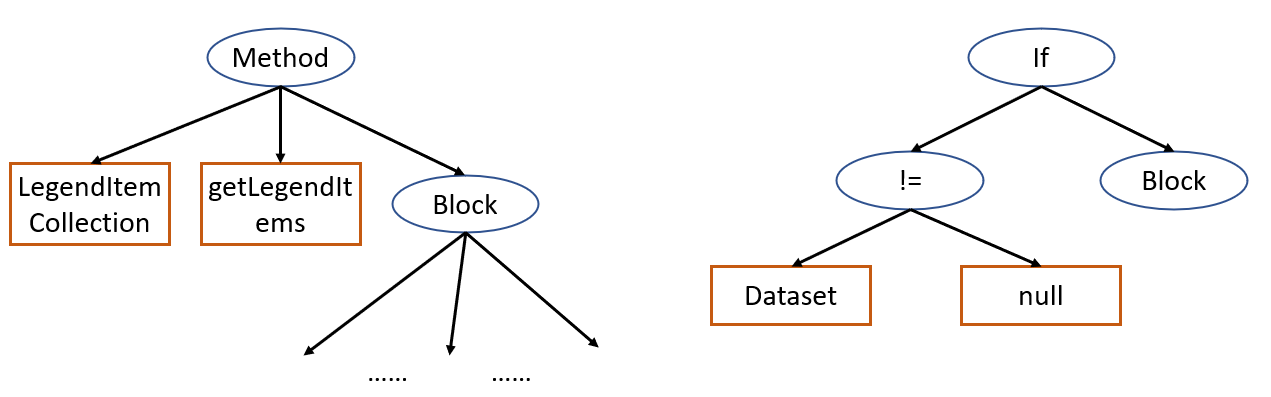
\includegraphics[width=3.2in]{graphs/tree_extraction.png}
%	\caption{Abstract Syntax Tree Extraction Example}
%	\label{tree-extraction}
%\end{figure}

The goal of this step is to take the source code under study and to
build the vector representations (embeddings).

\subsection{AST Building and Pairing of Subtrees}

First, for a buggy method $M$, we
%use Java JDT~\cite{JDT} to
parse the code to produce the AST for $M$. We also identify the
subtree $T_s$ corresponding to each buggy statement $s$. If there are
multiple buggy statements in $M$, we generate multiple AST subtrees
for them.  We use each buggy statement together with $M$
as a training instance for CCL and CTL.
%to train the context learning and code transformation models.

Second, to train CCL, we take a buggy method $M$ and the corresponding
fixed version of $M$, and parse them to build the two ASTs.
%
%we need the two ASTs for the buggy method $M$ and the corresponding
%fixed version of $M$. It is straightforward to collect them in the
%training dataset and build the ASTs before and after the fix.
However, to train CTL, as shown in Figure~\ref{overview-training}, we
need to identify the respective fixed subtree for the subtree $T_s$ of
a buggy statement. To do so, we use the tree differencing tool,
CPatMiner~\cite{nguyen2019graph}, to derive the fixing changes. If a
subtree corresponds to a statement, let us call it {\em
  S-subtree}. From CPatMiner's result, we use the following rules to
{\em pair a buggy subtree with the corresponding fixed subtree}:

1. A buggy subtree ($S$-subtree) is a subtree with
\code{update} or \code{delete}.

2. If a $S$-subtree is \code{deleted}, we pair it with an empty tree.

3. If a buggy $S$-subtree is marked as \code{update}, (i.e, it is
{\em updated} or its children node(s) could be {\em inserted, deleted} or {\em
  updated}), we paired this buggy $S$-subtree with its corresponding
fixed $S$-subtree.
%produced by CPatMiner.

4. If a $S$-subtree is \code{inserted} and its parent node is another
$S$-subtree, we pair it with that parent $S$-subtree.  If the parent
node is not an $S$-subtree, we pair an empty tree to the corresponding
inserted $S$-subtree.

%The first step of the \tool is the tree extraction step designed to extract abstract syntax tree (AST) from the source code. It accepts the buggy method with the changed statements inside as input. The output of this step is the extracted AST for the whole buggy method and the extracted subtree of AST that represents the changed statements.

%Specifically, for a buggy method $m$, \tool uses the Java package JDT \cite{JDT} to generate the AST $Tree_m$ to represent the buggy method. And for a buggy statement $s$ in the buggy method, \tool uses the subtree of AST $Tree_s$ that exactly covers the statement $s$ to represent the buggy statement. For example, in Figure \ref{tree-extraction}, the AST in the left represents the buggy method in Figure \ref{fig:motiv}, and the right subtree of AST in Figure \ref{tree-extraction} represents the buggy statement. If there is more than one buggy statement in the buggy method $m$, \tool generates multiple subtree of AST to represent each buggy statement.

%Also, when training the model, \tool needs ground truth to let the model learn the parameters, \tool also generates the AST $Tree_{mf}$ to represent the fixed method $m_f$ and the subtree of AST $Tree_{sf}$ to represent the fixed statement $s_f$. Here, $m_f$ is the after fixing version of buggy method $m$, and $s_f$ is the after fixing version of buggy statement $s$. Thus, \tool uses the AST and subtree of AST for fixed method and fixed statement as the ground truth to train the model parameters.

%For the buggy method, $m$ and corresponding fixed method $m_f$, \tool can easily find them from the dataset based on the true labels. However, pairing the buggy statement $s$ with its corresponding fixed version $s_f$ is not easy as the methods. To solve this problem, we use an existing approach CPatMiner \cite{nguyen2019graph} to process the fixing changes. Based on the results from CPatMiner, we pair the buggy statement $s$ with the corresponding fixed statement $s_f$ within the three following conditions. 1) If the buggy statement $s$ needs to be deleted, we pair $s$ with an empty statement. 2) if the buggy statement $s$ needs to be updated, we pair $s$ with the updated statement. 3) If there needs to insert a new statement as the fixing, we check the AST for the method $m$ first. And we pair the parent node with the inserted statement $s_f$ if the parent node representing the other statement, or we pair an empty statement with the inserted statement $s_f$.

\subsection{AST Node Representation Learning}

To provide the compatible inputs for CCL and CTL models, we need to
perform an AST node representation learning process in which each node
in the AST subtree or the AST of the method is replaced by the vector
representation (embedding) of the node. To achieve that, we first
flatten the abstract syntax (sub)tree under study by a
depth-first-search traversal to obtain a sequence of tokens. For the
case of an AST subtree, we consider the sequence of tokens of a
$S$-subtree as a sentence. For the case of the AST of the method, we
consider the sequence of tokens for the method as a sentence. We then
use the word embedding technique GloVe~\cite{pennington2014glove}
to run on those sentences to build a vector representation for each
token, i.e., for each AST node in the method's AST or in the AST
subtree. We used GloVe because it can capture well the co-occurrences
among tokens~\cite{pennington2014glove}. After running GloVe, we
replace each node in the (sub)tree with its GloVe vector
representation (see Figures~\ref{overview-training}
and~\ref{overview-fixing}). Similarly, we replace each node with its
vector in the AST of the fixed method and in the AST subtree of the
fixed~statement.

%To make the dual learning program repair model can take information from the input, \tool firstly needs to vectorize the AST and the subtree of AST by using the node representation learning.

%For a given tree $T$, \tool firstly uses the deep traversal to covert it into a sequence of tokens $S$. Here, $T$ could be $Tree_m$, $Tree_{mf}$, $Tree_s$, and $Tree_{sf}$. And then, \tool uses the famous technique GloVe \cite{pennington2014glove} to transform each AST node into a vector. The GloVe is a great tool for vectorizing the sequence of tokens by considering co-occurrence between different tokens. It can help predict for the often appeared together tokens. That's the reason why to choose it here to vectorize the tree $T$. For example, in Figure \ref{program-repair}, the AST node $N1-N5$ has been embedded into the vector $V1-V5$ in the top raw.
